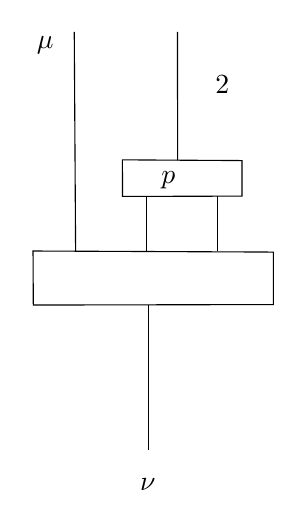
\begin{tikzpicture}[yscale=-1,scale=0.03,baseline={([yshift=-.5ex]current bounding box.center)}]
\begin{scope}[shift={(0.00mm,719.29mm)}]
% path id='path4136'
% path spec='m 348.3188,211.44613 1.19398,228.76363 1016.21342,-2.0203 0,-222.23354 z'
\draw [fill=none,draw=black] (348.32mm,211.45mm)
-- ++(1.19mm,228.76mm)
-- ++(1016.21mm,-2.02mm)
-- ++(0.00mm,-222.23mm)
-- cycle
;
% path id='path4138'
% path spec='m 828.55173,-20.130368 7.3e-4,232.485098'
\draw [fill=none,draw=black] (828.55mm,-20.13mm)
-- ++(0.00mm,232.49mm)
;
% path id='path4140'
% path spec='m 1128.5904,-20.487511 7e-4,232.842241'
\draw [fill=none,draw=black] (1128.59mm,-20.49mm)
-- ++(0.00mm,232.84mm)
;
% path id='path4142'
% path spec='m 522.85714,-716.2092 5.71429,928.57142'
\draw [fill=none,draw=black] (522.86mm,-716.21mm)
-- ++(5.71mm,928.57mm)
;
% path id='path4144'
% path spec='m 835.71429,438.07646 0,614.28584'
\draw [fill=none,draw=black] (835.71mm,438.08mm)
-- ++(0.00mm,614.29mm)
;
\node [black] at (400mm,-658.38mm) { $\mu$ };
\node [black] at (834.39mm,1200mm) { $\nu$ };
% path id='path4229'
% path spec='m 726.67898,-174.47875 0.59428,154.898727 505.80544,-1.36797 0,-150.477117 z'
\draw [fill=none,draw=black] (726.68mm,-174.48mm)
-- ++(0.59mm,154.90mm)
-- ++(505.81mm,-1.37mm)
-- ++(0.00mm,-150.48mm)
-- cycle
;
\node [black] at (921.43mm,-87.64mm) { $p$ };
% path id='path4235'
% path spec='m 960.48361,-172.13017 -0.66849,-544.64615 0,0'
\draw [fill=none,draw=black] (960.48mm,-172.13mm)
-- ++(-0.67mm,-544.65mm)
-- ++(0.00mm,0.00mm)
;
\node [black] at (1150mm,-493.35mm) { $\ydiagram{2}$ };
\end{scope}
\end{tikzpicture}
